Além disso, três abordagens podem ser tomadas em relação aos sinais aplicados para gerar os passos do motor.

\subsubsection{Passo Completo}

Os motores híbridos padrão possuem 200 passos completos por rotação do eixo do motor. Dividindo os número de passos por uma rotação completa ($360^{\circ}$) obtêm-se o ângulo de passo completo de $1,8^{\circ}$. Na maioria das vezes alcança-se o modo de passo completo ao energizar ambos os enrolamentos e inverter a corrente de forma alternada. 

\begin{figure}[ht!]
    \center 
    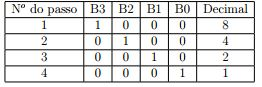
\includegraphics[scale=1]{imagens/f19}
    \caption{Controle Passo Completo 1}
\end{figure}


\begin{figure}[ht!]
    \center 
    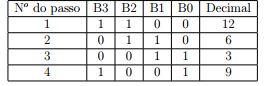
\includegraphics[scale=1]{imagens/f20}
    \caption{Controle Passo Completo 2}
\end{figure}
    
\subsubsection{Meio Passo}

Neste caso o motor vai girar 400 passos por rotação. Primeiro um enrolamento é energizado para depois dois enrolamentos serem energizados de forma alternada. Isso faz com que o mesmo gire por metade da distância ou $0,9^{\circ}$. Este tipo de configuração terá um movimento mais suave, porém com menos torque quando comparado com o passo completo. 

\begin{figure}[ht!]
    \center 
    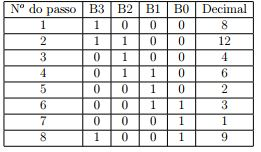
\includegraphics[scale=1]{imagens/f21}
    \caption{Controle Meio Passo}
\end{figure}
    
\subsubsection{Micro-passo}

Esta configuração controla a corrente no enrolamento do motor a um determinado grau que chega a subdividir o número das posições entre os polos. Existem modelos que são capazes de dividir um passo completo em 256 micro-passos ou seja $0,007^{\circ}$/passo. É utilizado em aplicações que necessitam de grande precisão para altas velocidades.

